\documentclass[11pt, a4paper]{report}

% ========== Common Packages ==========
\usepackage{fontspec}
\usepackage{kotex}
\usepackage{amsmath, amssymb, amsthm}
\usepackage{mathtools}
\usepackage{bm}
\usepackage{graphicx}
\usepackage{booktabs}
\usepackage{array}
\usepackage{tabularx}
\usepackage{longtable}
\usepackage{hyperref}
\usepackage{cleveref}
\usepackage{geometry}
\usepackage{fancyhdr}
\usepackage{titlesec}
\usepackage{enumitem}
\usepackage{xcolor}
\usepackage{tcolorbox}
\usepackage{algorithm}
\usepackage{algorithmic}
\usepackage{tikz}
\usetikzlibrary{arrows.meta, positioning, calc, decorations.pathreplacing, shapes.geometric, fit, patterns, angles, quotes, trees}
\usepackage{pgfplots}
\pgfplotsset{compat=1.18}
\usepackage{caption}
\usepackage{subcaption}
\usepackage{float}

\geometry{margin=2.5cm, top=3cm, bottom=3cm}

\usepackage{multirow}
\usepackage{siunitx}
% ========== Colors ==========
% Common
\definecolor{defblue}{RGB}{30, 80, 150}
\definecolor{thmgreen}{RGB}{20, 110, 60}
\definecolor{noteorange}{RGB}{200, 100, 0}
\definecolor{lightblue}{RGB}{230, 240, 255}
\definecolor{lightgreen}{RGB}{230, 255, 235}
\definecolor{lightorange}{RGB}{255, 245, 230}
\definecolor{lightgray}{RGB}{245, 245, 245}
% Extended
\definecolor{lightred}{RGB}{255, 235, 235}
\definecolor{darkred}{RGB}{180, 30, 30}
\definecolor{biogreen}{RGB}{10, 130, 80}
\definecolor{cvpurple}{RGB}{100, 40, 150}
\definecolor{injuryred}{RGB}{200, 40, 40}
\definecolor{codegray}{RGB}{240, 240, 245}
\definecolor{pipeblue}{RGB}{25, 100, 180}
\definecolor{constraintred}{RGB}{200, 50, 50}
\definecolor{termblack}{RGB}{30, 30, 30}
\definecolor{goldcolor}{RGB}{180, 140, 20}

% ========== Theorem-like environments ==========
\theoremstyle{definition}
\newtheorem{definition}{Definition}[chapter]
\newtheorem{example}{Example}[chapter]

\theoremstyle{plain}
\newtheorem{theorem}{Theorem}[chapter]
\newtheorem{proposition}{Proposition}[chapter]

\theoremstyle{remark}
\newtheorem{remark}{Remark}[chapter]

% ========== tcolorbox environments ==========
% --- Common (all parts) ---
\newtcolorbox{keyidea}[1][]{
  colback=lightblue,
  colframe=defblue,
  fonttitle=\bfseries,
  title={Key Idea},
  #1
}

\newtcolorbox{importantnote}[1][]{
  colback=lightorange,
  colframe=noteorange,
  fonttitle=\bfseries,
  title={Important},
  #1
}

\newtcolorbox{summary}[1][]{
  colback=lightgreen,
  colframe=thmgreen,
  fonttitle=\bfseries,
  title={Summary},
  #1
}

% --- Warning/Error ---
\newtcolorbox{warningbox}[1][]{
  colback=lightred,
  colframe=darkred,
  fonttitle=\bfseries,
  title={Warning},
  #1
}

% --- Domain: Biomechanics & Clinical ---
\newtcolorbox{clinicalnote}[1][]{
  colback=lightred,
  colframe=darkred,
  fonttitle=\bfseries,
  title={Clinical Note},
  #1
}

\newtcolorbox{biomechbox}[1][]{
  colback=lightgreen,
  colframe=biogreen,
  fonttitle=\bfseries,
  title={Biomechanics},
  #1
}

\newtcolorbox{injurybox}[1][]{
  colback={injuryred!8},
  colframe=injuryred,
  fonttitle=\bfseries,
  title={Injury Risk},
  #1
}

% --- Domain: Computer Vision ---
\newtcolorbox{cvbox}[1][]{
  colback={cvpurple!5},
  colframe=cvpurple,
  fonttitle=\bfseries,
  title={Computer Vision},
  #1
}

% --- Pipeline & Setup ---
\newtcolorbox{setupbox}[1][]{
  colback=lightgray,
  colframe=gray!60,
  fonttitle=\bfseries,
  title={Setup},
  #1
}

\newtcolorbox{pipelinebox}[1][]{
  colback=pipeblue!5,
  colframe=pipeblue,
  fonttitle=\bfseries,
  title={Pipeline Step},
  #1
}

\newtcolorbox{codebox}[1][]{
  colback=codegray,
  colframe=gray!70,
  fonttitle=\bfseries\ttfamily,
  title={Code},
  #1
}

\newtcolorbox{termbox}[1][]{
  colback=termblack!5,
  colframe=termblack!60,
  fonttitle=\bfseries\ttfamily,
  title={Terminal},
  #1
}

% --- Research ---
\newtcolorbox{hypothesis}[1][]{
  colback=goldcolor!8,
  colframe=goldcolor,
  fonttitle=\bfseries,
  title={Hypothesis},
  #1
}

\newtcolorbox{resultbox}[1][]{
  colback=thmgreen!8,
  colframe=thmgreen,
  fonttitle=\bfseries,
  title={Expected Result},
  #1
}

% --- Constraints & Solutions ---
\newtcolorbox{constraintbox}[1][]{
  colback=constraintred!8,
  colframe=constraintred,
  fonttitle=\bfseries,
  title={Constraint},
  #1
}

\newtcolorbox{solutionbox}[1][]{
  colback=thmgreen!8,
  colframe=thmgreen,
  fonttitle=\bfseries,
  title={Solution},
  #1
}

\newtcolorbox{databox}[1][]{
  colback=pipeblue!5,
  colframe=pipeblue,
  fonttitle=\bfseries,
  title={Data Spec},
  #1
}

% --- Progress/Status ---
\newtcolorbox{successbox}[1][]{
  colback=lightgreen,
  colframe=thmgreen,
  fonttitle=\bfseries,
  title={Success},
  #1
}

\newtcolorbox{nextbox}[1][]{
  colback=lightorange,
  colframe=noteorange,
  fonttitle=\bfseries,
  title={Next Step},
  #1
}

% --- Fitting guide ---
\newtcolorbox{failbox}[1][]{
  colback=lightred,
  colframe=darkred,
  fonttitle=\bfseries,
  title={Failure Pattern},
  #1
}

\newtcolorbox{fixbox}[1][]{
  colback=lightgreen,
  colframe=thmgreen,
  fonttitle=\bfseries,
  title={Fix},
  #1
}

\newtcolorbox{lessonbox}[1][]{
  colback=lightorange,
  colframe=noteorange,
  fonttitle=\bfseries,
  title={Lesson Learned},
  #1
}

% --- Specification ---
\newtcolorbox{specbox}[1][]{
  colback=cvpurple!5,
  colframe=cvpurple,
  fonttitle=\bfseries,
  title={Specification},
  #1
}

\newtcolorbox{checklistbox}[1][]{
  colback=lightgreen,
  colframe=biogreen,
  fonttitle=\bfseries,
  title={Checklist},
  #1
}

% ========== Custom math commands ==========
% Vectors (lowercase)
\newcommand{\vx}{\mathbf{x}}
\newcommand{\vd}{\mathbf{d}}
\newcommand{\vo}{\mathbf{o}}
\newcommand{\vc}{\mathbf{c}}
\newcommand{\vr}{\mathbf{r}}
\newcommand{\vp}{\mathbf{p}}
\newcommand{\vv}{\mathbf{v}}
\newcommand{\vn}{\mathbf{n}}
\newcommand{\vu}{\mathbf{u}}
\newcommand{\vt}{\mathbf{t}}
\newcommand{\ve}{\mathbf{e}}
\newcommand{\vq}{\mathbf{q}}
% Vectors (uppercase)
\newcommand{\vF}{\mathbf{F}}
\newcommand{\vM}{\mathbf{M}}
\newcommand{\va}{\mathbf{a}}
\newcommand{\vg}{\mathbf{g}}
\newcommand{\vX}{\mathbf{X}}
% Bold Greek
\newcommand{\vmu}{\bm{\mu}}
\newcommand{\vbeta}{\bm{\beta}}
\newcommand{\vtheta}{\bm{\theta}}
\newcommand{\vpsi}{\bm{\psi}}
% Matrices
\newcommand{\mSigma}{\bm{\Sigma}}
\newcommand{\mR}{\mathbf{R}}
\newcommand{\mS}{\mathbf{S}}
\newcommand{\mW}{\mathbf{W}}
\newcommand{\mJ}{\mathbf{J}}
\newcommand{\mG}{\mathbf{G}}
\newcommand{\mT}{\mathbf{T}}
\newcommand{\mI}{\mathbf{I}}
\newcommand{\mB}{\mathbf{B}}
\newcommand{\mK}{\mathbf{K}}
\newcommand{\mP}{\mathbf{P}}
\newcommand{\mF}{\mathbf{F}}
\newcommand{\mE}{\mathbf{E}}
\newcommand{\mA}{\mathbf{A}}
\newcommand{\mH}{\mathbf{H}}
% Sets and groups
\newcommand{\RR}{\mathbb{R}}
\newcommand{\SO}{\mathrm{SO}}
% Units
\newcommand{\degps}{\,\text{deg/s}}
\newcommand{\Nm}{\ensuremath{\,\text{N}\cdot\text{m}}}
\newcommand{\BW}{\,\text{BW}}

% ========== Header/Footer ==========
\pagestyle{fancy}
\fancyhf{}
\fancyhead[L]{\leftmark}
\fancyhead[R]{\thepage}
\renewcommand{\headrulewidth}{0.4pt}

% ========== Title formatting ==========
\titleformat{\chapter}[display]
  {\normalfont\huge\bfseries\color{defblue}}
  {\chaptertitlename\ \thechapter}{20pt}{\Huge}

\titleformat{\section}
  {\normalfont\Large\bfseries\color{defblue!80!black}}
  {\thesection}{1em}{}

\titleformat{\subsection}
  {\normalfont\large\bfseries\color{defblue!60!black}}
  {\thesubsection}{1em}{}


\begin{document}

\begin{titlepage}
\centering
\vspace*{1.5cm}
{\Large\color{gray} Experiment Log Day 3}
\vspace{0.5cm}

{\Huge\bfseries\color{defblue} 2026년 4월 13--14일\\[0.3cm]
GART 설치 완료 $\rightarrow$ 4뷰 1000프레임\\[0.3cm]
파이프라인 구축}

\vspace{1cm}

{\LARGE\color{defblue!70!black} GART 공식 install.sh 방식 설치 성공\\
U-HMR 4뷰 $\rightarrow$ 4뷰 Sequential Reproj\\
$\rightarrow$ GART 4뷰 1000프레임 학습}

\vspace{2cm}
{\large 2026년 4월 14일}
\end{titlepage}

\tableofcontents
\newpage


% ====================================================================
\chapter{GART 설치}
% ====================================================================

\section{공식 install.sh 방식}

기존: 임의 패키지 설치로 반복 충돌. 해결: GART의 공식 \texttt{install.sh} 순서를 정확히 따름.

\begin{table}[H]
\centering
\caption{GART conda 환경 최종 구성}
\renewcommand{\arraystretch}{1.3}
\begin{tabular}{l l l}
\toprule
\textbf{패키지} & \textbf{버전} & \textbf{설치 방법} \\
\midrule
Python & 3.9 & conda create \\
PyTorch & 2.0.0+cu118 & conda (pytorch channel) \\
pytorch3d & 0.7.7 & conda (pytorch3d channel) \\
cuda-toolkit & 11.8 & conda (nvidia channel) \\
cuda-nvcc & 11.8.89 & conda (nvidia channel) \\
simple-knn & 소스 빌드 & pip --no-build-isolation \\
diff\_gaussian\_rasterization & 소스 빌드 & pip --no-build-isolation \\
smplx & 0.1.28 + shim & pip \\
numpy & 1.26.4 & pip \\
\bottomrule
\end{tabular}
\end{table}

\section{해결한 문제들}

\begin{enumerate}[leftmargin=*]
  \item \textbf{nvcc 12.4 $\rightarrow$ 11.8}: \texttt{cuda-toolkit=11.8}만으로는 시스템 nvcc(12.4)가 우선됨. \texttt{cuda-nvcc=11.8.89}를 별도 설치하여 해결.
  \item \textbf{cub/cub.cuh 미발견}: CUDA 11.8에서 CUB 헤더 경로가 다름. \texttt{CPATH=\$CONDA\_PREFIX/targets/x86\_64-linux/include} 설정.
  \item \textbf{FLT\_MAX 미정의}: \texttt{simple\_knn.cu}에 \texttt{\#include <cfloat>} 추가.
  \item \textbf{PEP-517 빌드 격리}: pip의 빌드 격리 환경에서 torch를 못 찾음. \texttt{--no-build-isolation}으로 해결 (install.sh 작성 시점의 pip 동작과 동일).
  \item \textbf{smplx shim}: \texttt{smplx.smplx} 모듈 생성, \texttt{templates.py}의 \texttt{.J/.A} 수동 계산.
  \item \textbf{빈 마스크 crash}: \texttt{get\_bbox}와 \texttt{voxel\_deformer}에 빈 텐서 가드 추가.
\end{enumerate}


% ====================================================================
\chapter{파이프라인 구조 변경: 7뷰 $\rightarrow$ 4뷰}
% ====================================================================

\section{문제: 뷰 불일치}

\begin{warningbox}
이전 시도에서 U-HMR은 \textbf{4뷰}(cam3,5,6,7)로 body\_pose를 추출했지만, reproj는 \textbf{7뷰}, GART는 \textbf{6뷰}(cam1 세로 제외)로 진행하면서 불일치 발생.

결과: reproj 에러 160$\sim$1100px (중반 이후 폭발), GART 렌더링 블러.
\end{warningbox}

\section{해결: 4뷰 일관 파이프라인}

\begin{keyidea}
U-HMR이 실제로 본 카메라와 동일한 4뷰만 사용:
\[
\text{U-HMR 4뷰} \xrightarrow{\text{body\_pose}} \text{Reproj 4뷰} \xrightarrow{\text{Rh, Th}} \text{GART 4뷰}
\]
cam3, cam5, cam6, cam7 --- 모두 1920$\times$1080, 1000프레임.
\end{keyidea}

추가 문제 해결:
\begin{itemize}[leftmargin=*]
  \item cam1 세로 방향(1080$\times$1920) $\rightarrow$ 제외
  \item macOS \texttt{.\_} 리소스 포크 파일 $\rightarrow$ 필터링
  \item 배치 reproj에서 모든 프레임이 같은 초기값 $\rightarrow$ Sequential fitting으로 변경
\end{itemize}


% ====================================================================
\chapter{4뷰 Sequential Reprojection 피팅}
% ====================================================================

\section{방법}

\begin{enumerate}[leftmargin=*]
  \item 프레임별 U-HMR body\_pose를 초기값으로 사용 (\texttt{uhmr\_all\_frames/})
  \item \textbf{Sequential}: 이전 프레임의 Rh, Th를 다음 프레임 초기값으로 전파
  \item Stage 1: Rh(3) + Th(3) 최적화 (80 steps, lr=0.05)
  \item Stage 2: + body\_pose fine-tune (40 steps, lr=0.008, regularization)
  \item 4카메라 2D keypoint(OpenPose smoothed v2) + GMoF robust loss
\end{enumerate}

\section{결과}

\begin{table}[H]
\centering
\caption{Reproj 에러 비교 (px/frame)}
\renewcommand{\arraystretch}{1.3}
\begin{tabular}{l ccc}
\toprule
& \textbf{7뷰 Batch} & \textbf{4뷰 Sequential} & \textbf{개선} \\
\midrule
Mean reproj & 354.9 px & \textbf{153.5 px} & 57\% $\downarrow$ \\
Median reproj & --- & \textbf{153.6 px} & --- \\
$<$200px 비율 & 불안정 & \textbf{956/1000 (96\%)} & --- \\
안정성 & 160$\rightarrow$1100px 폭발 & 123$\sim$199px 일관적 & --- \\
\bottomrule
\end{tabular}
\end{table}

\begin{table}[H]
\centering
\caption{프레임 구간별 reproj 에러}
\renewcommand{\arraystretch}{1.3}
\begin{tabular}{l c}
\toprule
\textbf{프레임 구간} & \textbf{Reproj (px)} \\
\midrule
0--100 & 173.8 $\rightarrow$ 153.9 \\
100--300 & 160.7 $\sim$ 163.8 \\
300--500 & 163.2 $\sim$ 199.4 \\
500--700 & 136.0 $\sim$ 137.0 \\
700--900 & 137.0 $\sim$ 138.7 \\
900--1000 & 123.4 $\sim$ 204.2 \\
\bottomrule
\end{tabular}
\end{table}

\begin{keyidea}
Sequential fitting + 4뷰 일치로 전체 1000프레임에서 안정적인 reproj 달성. 특히 후반부(500+)에서 이전 7뷰 방식 대비 10배 이상 개선.
\end{keyidea}


% ====================================================================
\chapter{GART 학습 결과}
% ====================================================================

\section{6뷰 100프레임 (첫 번째 시도)}

\begin{itemize}[leftmargin=*]
  \item 입력: cam2--cam7, 100프레임, per-frame U-HMR body\_pose
  \item 3000 steps, $\sim$18 it/s, $\sim$3분
  \item 결과: 투수 실루엣 재구성 시작 (이전 1뷰에서는 빨간 배경만)
  \item Depth 맵에서 인체 형태가 정상적으로 추정됨
\end{itemize}

\begin{figure}[H]
\centering
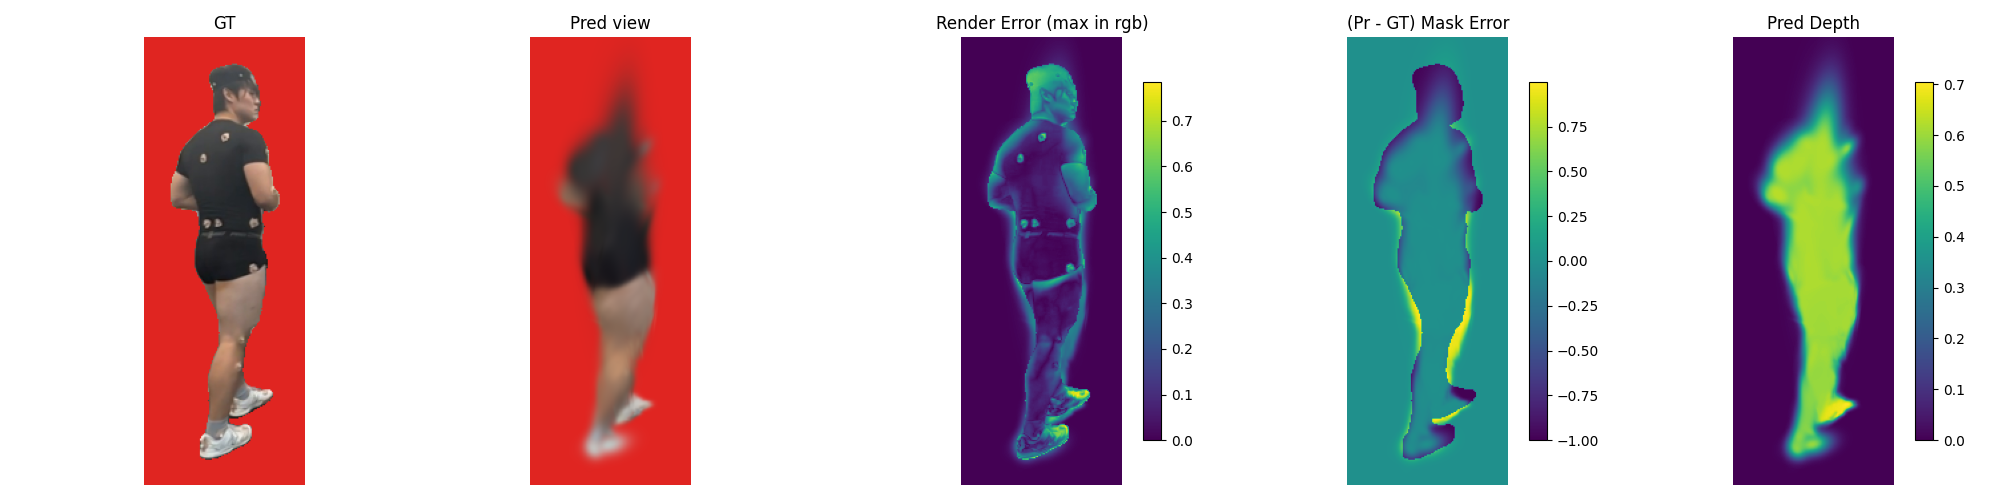
\includegraphics[width=\textwidth]{data/gart_7v_results/step_2999.png}
\caption{GART 6뷰 100프레임 Step 2999 결과. 좌: GT, Pred view에서 투수 실루엣이 보이기 시작. 이전 1뷰 결과(빨간 배경)에서 크게 개선.}
\end{figure}

\section{4뷰 1000프레임 (최종)}

\begin{itemize}[leftmargin=*]
  \item 입력: cam3, cam5, cam6, cam7 (U-HMR과 동일 4뷰)
  \item 1000프레임 $\times$ 4뷰 = 4000 이미지
  \item Sequential reproj로 정제된 SMPL 파라미터 사용
  \item 3000 steps 학습
\end{itemize}


% ====================================================================
\chapter{현재 상태 및 다음 단계}
% ====================================================================

\begin{table}[H]
\centering
\caption{파이프라인 진행 상황}
\renewcommand{\arraystretch}{1.4}
\begin{tabular}{c p{5cm} c p{4cm}}
\toprule
\textbf{Step} & \textbf{작업} & \textbf{상태} & \textbf{비고} \\
\midrule
1 & GART 공식 설치 & \textbf{완료} & conda, nvcc 11.8 \\
2 & U-HMR 999프레임 추론 & \textbf{완료} & 4뷰, 18분 \\
3 & OpenPose smoothing v2 & \textbf{완료} & 7대, 83--87\% 감소 \\
4 & 4뷰 Sequential Reproj & \textbf{완료} & 1000프레임, mean 153px \\
5 & GART 4뷰 데이터 준비 & \textbf{완료} & ZJU-MoCap 형식 \\
6 & GART 4뷰 학습 & \textbf{진행중} & 1000프레임, 3000 steps \\
7 & 생체역학 분석 & 대기 & SMPL2AddBiomechanics \\
\bottomrule
\end{tabular}
\end{table}

\begin{summary}
\textbf{핵심 성과}:
\begin{enumerate}[leftmargin=*]
  \item GART 공식 install.sh 방식 설치 성공 (nvcc 11.8, CUDA 확장 빌드)
  \item 7뷰 $\rightarrow$ 4뷰 일관 파이프라인으로 구조 개선
  \item Sequential reproj로 1000프레임 안정적 피팅 (mean 153px, 96\% $<$ 200px)
  \item GART 6뷰에서 투수 형태 첫 재구성
  \item 4뷰 1000프레임 GART 학습 실행
\end{enumerate}

\textbf{남은 과제}:
\begin{enumerate}[leftmargin=*]
  \item Reproj 에러 추가 감소 (153px $\rightarrow$ $<$50px)
  \item GART steps 증가 (3000 $\rightarrow$ 15000+)
  \item 렌더링 품질 검증
  \item 생체역학 분석 파이프라인 연결
\end{enumerate}
\end{summary}


\end{document}
